\chapter{Background}
%\label{chap:intro}


This chapter presents a briefly theoretical background that is needed in order to understand the thesis. To fully understand any topic, the reader should refer to the reference.


\section{ROS: Robotic Operating System}

ROS is a flexible framework for writing robot software. It is a collection of tools, libraries, and conventions that aim to simplify the task of creating complex and robust robot behaviour across a wide variety of robotic platforms. It is based on the concepts of nodes, topics, messages and services. A node is an executable program that performs computation. Nodes need to communicate with each other to complete the whole task. The communicated data are called messages. ROS provides an easy way for passing messages and establishing communication links between nodes, which are running independently. They pass these messages to each other over a Topic, which is a simple string. However, topics are asynchronous, synchronous communication is provided by services. Services act in a call-response manner where one node requests that another node execute a one-time computation and provide a response. For more details about ROS, the reader can refer to \cite{ros}.

\begin{figure}[!h]
\begin{center}
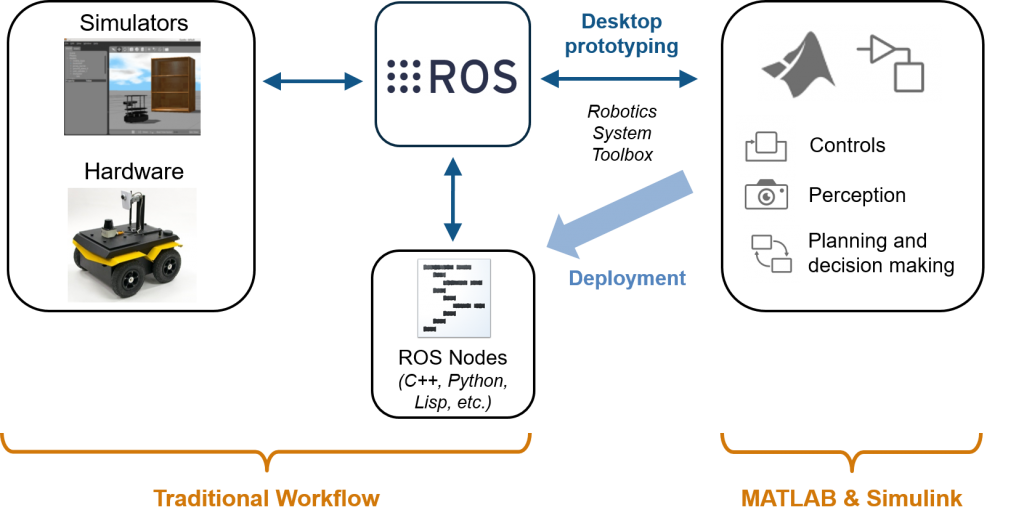
\includegraphics[width=2in]{figures02/ros_workflows}
\caption{A ROS Overview}%\cite{temp2}}
\end{center}
%\label{fig2:mypicture3}
\end{figure}
